\chapter{Conexión}

\section{Conjuntos conexos}

Los espacios \textit{conexos} vendrían a ser espacios que están ``conectados'' ---valga la redundancia---. En particular, se nos va a hacer más fácil definir la no-conexión.

\begin{definition}
	Sea $(X, d)$ un espacio métrico. Decimos que $X$ \textbf{no} es \emph{conexo} si se cumple alguna de las siguientes:
	\begin{enumerate}
		\item Existe $B \subseteq X$ abierto y cerrado tal que $B \neq X$.
		\item Existen $U, V \subseteq X$ abiertos disjuntos no vacíos tales que $U \cup V = X$.
		\item Existen $A, B \subseteq X$ cerrados disjuntos no vacíos tales que $A \cup B = X$.
	\end{enumerate}
\end{definition}

\begin{remark}
	Las condiciones 1., 2. y 3. son equivalentes.
\end{remark}

\begin{proof}
	Sea $(X, d)$ un espacio métrico.

	(1 $\Rightarrow$ 2) Supongamos que existe $B \subseteq X$ abierto y cerrado no vacío tal que $B \neq X$. Consideramos $B \cup (X \setminus B) = X$ y basta con ver que ambos subconjuntos son abiertos, disjuntos y no vacíos. Por hipótesis, $B$ es abierto; como también es cerrado, entonces $X \setminus B$ es abierto. Como $B$ es un subconjunto propio de $X$, entonces su complemento es no vacío.

	(2 $\Rightarrow$ 3) Supongamos que existen $U, V \subseteq X$ abiertos disjuntos no vacíos tales que $U \cup V = X$. Consideramos $A = X \setminus U$ y $B = X \setminus V$. Ambos son cerrados al ser complementos de abiertos. Dado que $U \cup V = X$, obtenemos que $A \cap B = \varnothing$, por ende son disjuntos. Veamos que su unión es $X$. Sea $x \in X$. Entonces, o bien $x \in U$ o $x \in V$. Si $x \in U$, entonces $x \not \in V$, por lo tanto $x \in X \setminus V = B$. Análogamente, Si $x \in V$, entonces $x \not \in U$, por lo tanto $x \in X \setminus U = A$. Lo cual nos dice que $X = A \cup B$.

	(3 $\Rightarrow$ 1) Supongamos que existen $A, B \subseteq X$ cerrados disjuntos no vacíos tales que $A \cup B = X$. Como $A \cup B = X$, obtenemos que $B = X \setminus A$. Dado que $A$ y $B$ son disjuntos no vacíos, $B \neq X$. También, $B$ es cerrado y, como es el complemento de un cerrado, $B$ es abierto.
\end{proof}

Ahora sí definimos conexión.

\begin{definition}
	Sea $(X, d)$ un espacio métrico. Decimos que $X$ es \emph{conexo} si no se cumple ninguna de las propiedades anteriores.
\end{definition}

Algunos ejemplos.

\begin{example}
	\begin{enumerate}
		\item Los intervalos de $\mathbb{R}$ son conexos.
		\item Las bolas en $\mathbb{R}^n$ son conexas.
		\item El espacio con un elemento es conexo.
	\end{enumerate}
\end{example}

\section{Propiedades de conexos}

Vamos a caracterizar los conexos de $\mathbb{R}$, pero antes veamos un lema que nos va a ayudar.

\begin{lemma}
	Un subconjunto $X \subseteq \mathbb{R}$ es un intervalo si y sólo si, para todo $a, b \in X$ tales que $a \leq b$, se cumple que $[a, b] \subseteq X$.
\end{lemma}

\begin{proof}
	($\Rightarrow$) Sea $X \subseteq \mathbb{R}$ un intervalo con bordes en $x, y \in \mathbb{R}$ tal que $x \leq y$. Sean $a, b \in X$ tales que $a \leq b$. Sea $c \in [a, b]$. Como $x < a \leq c \leq b < y$, entonces $c \in X$. (La demostración es casi idéntica si el intervalo $X$ es abierto, semiabierto o cerrado.)

	($\Leftarrow$) Sea $X \subseteq \mathbb{R}$ tal que para todo $a, b \in X$ tales que $a \leq b$ se cumple que $[a, b] \subseteq X$. Consideramos $[\inf X, \sup X] \subseteq \mathbb{R}$. Todo $x \in X$ pertenece al intervalo. Sea $x \in [\inf X, \sup X]$. Entonces, si $x \not \in X$, como existen $a, b \in X$ tales que $a \leq x \leq b$, llegamos a un absurdo. (Lo mismo, la demostración es casi idéntica, pero técnicamente hay que separar por casos.)
\end{proof}

Veamos cómo son los conexos de $\mathbb{R}$.

\begin{theorem}
	Sea $X \subseteq \mathbb{R}$. Entonces, $X$ es conexo si y sólo si $X$ es un intervalo.
\end{theorem}

\begin{proof}
	($\Rightarrow$) Probamos por contrarrecíproco. Supongamos que $X$ no es un intervalo. Entonces, existen un $a, b \in X$ y $r \not \in X$ tales que $a < r < b$. Por lo tanto, $((\infty, r) \cap X) \cup ((r, \infty \cap X)) = X$, entonces $X$ no es conexo.
	($\Leftarrow$) Sea $X$ no conexo. Sean $A, B \subseteq X$ abiertos disjuntos no vacíos tales que $A \cup B = X$. Consideramos $a \in A$ y $b \in B$. Definimos $c = \sup \left\{ x \in [a, b] \cap A \right\}$. O bien $c \in A$ o $c \in B$. Si $c \in A$, entonces como $A$ es abierto, $c$ no es una cota superior. Si $c \in B$, entonces como $B$ es abierto, existe una cota superior menor que $c$.
\end{proof}

Las funciones continuas, al igual que con los compactos, manda conexos a conexos.

\begin{theorem}
	Sea $X$ un espacio métrico conexo e $Y$ un espacio métrico. Sea $f : X \to Y$ continua. Entonces, $f(X)$ es conexo.
\end{theorem}

\begin{proof}
	Supongamos que $f(X)$ no es conexo. Entonces, existen $A, B \subseteq Y$ abiertos disjuntos no vacíos tales que $f(X) = A \cup B$. Tomando preimagen, $X = f^{-1}(A) \cup f^{-1}(B)$, donde $f^{-1}(A)$ y $f^{-1}(B)$ son abiertos disjuntos no vacíos. Esto implica que $X$ no es conexo, lo cual es absurdo.
\end{proof}

Este teorema nos proporciona una nueva manera de demostrar que un espacio es conexo: probamos que es imagen de un conexo por una función continua.

La proposición de a continuación nos va a ser más útil adelante.

\begin{proposition}
	Sea $Y$ un espacio métrico. Sea $X \subseteq Y$ un subespacio métrico tal que existen $A, B \subseteq X$ abiertos disjuntos no vacíos tales que $A \cup B = X$. Entonces, existen $V_{A}, V_B \subseteq Y$ abiertos disjuntos no vacíos tales que $A = V_A \cap X$ y $B = V_B \cap X$.
\end{proposition}

\begin{proof}
	Como $A$ y $B$ son abiertos en la topología subespacio de $X$, existen abiertos $V_A, V_B \subseteq Y$ tales que $A = V_A \cap X$ y $B = V_B \cap X$.

	Ahora bien, puede pasar que $V_A \cap V_B \neq \varnothing$. Pero como $A \cap B = \varnothing$, tenemos que $(V_A \cap V_B) \cap X = \varnothing$.

	Queremos modificar $V_A$ y $V_B$ para que sean disjuntos en $Y$ sin cambiar su intersección con $X$. Definimos
	\[
		\widetilde{V}_A := V_A \setminus \overline{V_B}, \qquad \widetilde{V}_B := V_B \setminus \overline{V_A}.
	\]
	Ambos conjuntos son abiertos como diferencia de abierto menos cerrado.

	Veamos que siguen cortando a $X$ donde queremos. Como $A = V_A \cap X$ y $A \cap \overline{V_B} = \varnothing$, se sigue que
	\[
		\widetilde{V}_A \cap X = (V_A \setminus \overline{V_B}) \cap X = V_A \cap X = A.
	\]
	Análogamente, $\widetilde{V}_B \cap X = B$.

	Finalmente, veamos que $\widetilde{V}_A$ y $\widetilde{V}_B$ son disjuntos. Si $x \in \widetilde{V}_A \cap \widetilde{V}_B$, entonces $x \in V_A$ y $x \notin \overline{V_B}$, pero también $x \in V_B$ y $x \notin \overline{V_A}$, lo cual es absurdo ya que $x \in V_B$ implica $x \in \overline{V_B}$ y análogamente para $V_A$.

	Entonces, $\widetilde{V}_A$ y $\widetilde{V}_B$ son abiertos disjuntos tales que $A = \widetilde{V}_A \cap X$ y $B = \widetilde{V}_B \cap X$.
\end{proof}

Ahora vamos a ver otra forma de demostrar que un espacio métrico es conexo.

\begin{proposition}
	Sea $X$ un espacio métrico. Entonces, $X$ es conexo si y sólo si toda función $g : X \to \left\{ 0, 1 \right\}$ continua es constante.
\end{proposition}

\begin{proof}
	($\Rightarrow$) Sea $X$ conexo y sea $g : X \to \left\{ 0, 1 \right\}$ continua. Consideramos a las preimágenes $f^{-1}(0)$ y $f^{-1}(1)$. Sabemos que $f^{-1}(0)$ y $f^{-1}(1)$ son disjuntas. Por continuidad de $f$, también son cerradas. Por último, $f^{-1}(0) \cup f^{-1}(1) = X$. Entonces, para que $X$ sea conexo, necesariamente alguna de las preimágenes es vacío.

	($\Leftarrow$) Supongamos que toda función $g : X \to \left\{ 0, 1 \right\}$ continua es constante. Supongamos que $X$ no es conexo, entonces existe una separación con $U, V \subseteq X$ cerrados disjuntos no vacíos tales que $U \cup V = X$. Definimos $f : X \to \left\{ 0, 1 \right\}$ tal que $f(U) = \left\{ 0 \right\}$ y $f(V) = \left\{ 1 \right\}$. Esto es absurdo.
\end{proof}

El siguiente teorema nos da una condición para que la unión de conexos sea conexa. Pensemos por qué no vale en general que la unión de conexos sea conexa. La idea es que la unión de dos conexos que no se ``tocan'' no es conexa.

\begin{center}
	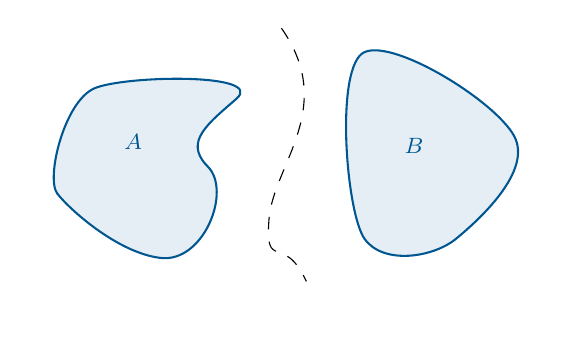
\begin{tikzpicture}[x=0.75pt,y=0.75pt,yscale=-1,xscale=1]
	%uncomment if require: \path (0,300); %set diagram left start at 0, and has height of 300

	%Shape: Polygon Curved [id:ds20022184980649105] 
	\draw  [color={rgb, 255:red, 0; green, 86; blue, 145 }  ,draw opacity=1 ][fill={rgb, 255:red, 0; green, 86; blue, 145 }  ,fill opacity=0.1 ][line width=0.75]  (47.85,39.3) .. controls (62.33,33.02) and (130.77,31.76) .. (116.3,44.33) .. controls (102.26,56.52) and (91.54,64.77) .. (101.55,75.96) .. controls (101.86,76.31) and (102.19,76.66) .. (102.54,77.01) .. controls (114.2,88.74) and (100.53,123.52) .. (79.7,121) .. controls (58.88,118.49) and (35.66,97.37) .. (30,90) .. controls (24.34,82.63) and (33.38,45.59) .. (47.85,39.3) -- cycle ;
	%Shape: Polygon Curved [id:ds5640401880667114] 
	\draw  [color={rgb, 255:red, 0; green, 86; blue, 145 }  ,draw opacity=1 ][fill={rgb, 255:red, 0; green, 86; blue, 145 }  ,fill opacity=0.1 ][line width=0.75]  (178.05,21.82) .. controls (192.52,15.53) and (240.75,45.29) .. (250.05,62.15) .. controls (259.34,79.02) and (233.05,102.82) .. (222.05,111.82) .. controls (211.05,120.82) and (187.05,124.48) .. (178.05,111.82) .. controls (169.05,99.15) and (163.57,28.1) .. (178.05,21.82) -- cycle ;
	%Curve Lines [id:da7601976291136298] 
	\draw  [dash pattern={on 4.5pt off 4.5pt}]  (138,10.33) .. controls (165,48.67) and (134,76.33) .. (132,102.33) .. controls (130,128.33) and (139,108.33) .. (150,132.33) ;

	% Text Node
	\draw (61,60) node [anchor=north west][inner sep=0.75pt]  [font=\footnotesize,color={rgb, 255:red, 0; green, 86; blue, 145 }  ,opacity=1 ]  {$A$};
	% Text Node
	\draw (196.05,62.02) node [anchor=north west][inner sep=0.75pt]  [font=\footnotesize,color={rgb, 255:red, 0; green, 86; blue, 145 }  ,opacity=1 ]  {$B$};
	% Text Node
	\draw (16,150) node [anchor=north west][inner sep=0.75pt]   [align=left] {};


\end{tikzpicture}

\end{center}

\begin{theorem}
	Sea $X$ un espacio métrico. Sea $\left\{ A_i \right\}_I$ una familia de subconjuntos conexos de $X$. Si existe $x \in X$ tal que, para todo $i \in I$, $x \in A_i$, entonces $\bigcup_{i \in I} A_i$ es conexo.
\end{theorem}

\begin{proof}
	Sea $g : \bigcup_{i \in I} A_j \to \left\{ 0, 1 \right\}$ una función continua cualquiera. Sea $x \in X$ tal que, para todo $i \in I$, $x \in A_i$. Entonces, consideramos $f(x)$. Si consideramos $f|_{A_i}$, entonces como es una función continua de un conexo a $\left\{ 0, 1 \right\}$, es constante. O sea, para todo $i \in I$, $f|_{A_i} = f(x)$. Entonces, $f$ es constante.
\end{proof}

\begin{remark}
	No hace falta que todos los conjuntos compartan un punto, con que para todo $\alpha, \beta \in I$, existan $i_1, i_2, \ldots, i_n \in I$ tales que
	\begin{equation*}
		A_{\alpha} \cap A_{i_1} \neq \varnothing, A_{i_1} \cap A_{i_2} \neq \varnothing, \ldots, A_{i_{n-1}} \cap A_{i_n} \neq \varnothing, A_{i_n} \cap A_{\beta} \neq \varnothing.
	\end{equation*}

	\begin{center}
		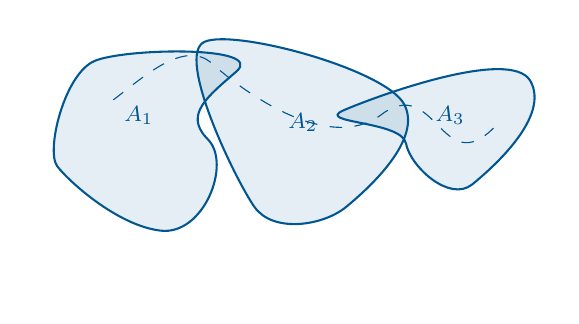
\begin{tikzpicture}[x=0.75pt,y=0.75pt,yscale=-1,xscale=1]
	%uncomment if require: \path (0,300); %set diagram left start at 0, and has height of 300

	%Shape: Polygon Curved [id:ds5691606692406826] 
	\draw  [color={rgb, 255:red, 0; green, 86; blue, 145 }  ,draw opacity=1 ][fill={rgb, 255:red, 0; green, 86; blue, 145 }  ,fill opacity=0.1 ][line width=0.75]  (47.85,39.3) .. controls (62.33,33.02) and (130.77,31.76) .. (116.3,44.33) .. controls (102.26,56.52) and (91.54,64.77) .. (101.55,75.96) .. controls (101.86,76.31) and (102.19,76.66) .. (102.54,77.01) .. controls (114.2,88.74) and (100.53,123.52) .. (79.7,121) .. controls (58.88,118.49) and (35.66,97.37) .. (30,90) .. controls (24.34,82.63) and (33.38,45.59) .. (47.85,39.3) -- cycle ;
	%Shape: Polygon Curved [id:ds015378215570174936] 
	\draw  [color={rgb, 255:red, 0; green, 86; blue, 145 }  ,draw opacity=1 ][fill={rgb, 255:red, 0; green, 86; blue, 145 }  ,fill opacity=0.1 ][line width=0.75]  (101,30) .. controls (115.48,23.72) and (187.75,43.14) .. (197.05,60) .. controls (206.34,76.86) and (180.05,100.67) .. (169.05,109.67) .. controls (158.05,118.67) and (134.05,122.33) .. (125.05,109.67) .. controls (116.05,97) and (86.52,36.28) .. (101,30) -- cycle ;
	%Shape: Polygon Curved [id:ds79267022071116] 
	\draw  [color={rgb, 255:red, 0; green, 86; blue, 145 }  ,draw opacity=1 ][fill={rgb, 255:red, 0; green, 86; blue, 145 }  ,fill opacity=0.1 ][line width=0.75]  (168,63) .. controls (182.48,56.72) and (248.7,32.14) .. (258,49) .. controls (267.3,65.86) and (241,89.67) .. (230,98.67) .. controls (219,107.67) and (200,90) .. (198,79) .. controls (196,68) and (153.52,69.28) .. (168,63) -- cycle ;
	%Curve Lines [id:da15620468455330305] 
	\draw [color={rgb, 255:red, 0; green, 86; blue, 145 }  ,draw opacity=1 ] [dash pattern={on 4.5pt off 4.5pt}]  (57,58) .. controls (71.07,47.45) and (91.29,28.38) .. (104.67,40.58) .. controls (118.04,52.78) and (160.24,84.53) .. (186.17,65.08) .. controls (212.1,45.64) and (215.17,96.58) .. (240.17,71.58) ;

	% Text Node
	\draw (61,60) node [anchor=north west][inner sep=0.75pt]  [font=\footnotesize,color={rgb, 255:red, 0; green, 86; blue, 145 }  ,opacity=1 ]  {$A_{1}$};
	% Text Node
	\draw (140.05,63.02) node [anchor=north west][inner sep=0.75pt]  [font=\footnotesize,color={rgb, 255:red, 0; green, 86; blue, 145 }  ,opacity=1 ]  {$A_{2}$};
	% Text Node
	\draw (16,150) node [anchor=north west][inner sep=0.75pt]   [align=left] {};
	% Text Node
	\draw (211,60) node [anchor=north west][inner sep=0.75pt]  [font=\footnotesize,color={rgb, 255:red, 0; green, 86; blue, 145 }  ,opacity=1 ]  {$A_{3}$};
\end{tikzpicture}

	\end{center}
\end{remark}

\begin{proposition}
	Sea $X$ un espacio métrico. Sea $A \subseteq X$ un subespacio métrico conexo denso. Entonces, $X$ es conexo.
\end{proposition}

\begin{proof}
	Sea $g : X \to \left\{ 0, 1 \right\}$ una función continua cualquiera. Entonces, $g|_A$ es constante. Por continuidad de $g$, la extensión de $g|_A$ a $X$ es igual a $g$. Por lo tanto, $g$ es constante y entonces $X$ es conexo.
\end{proof}

\begin{corollary}
	Sea $A$ conexo. Si $A \subseteq B \subseteq \overline{A}$, entonces $B$ es conexo.
\end{corollary}

\begin{proof}
	Como $B \subseteq \overline{A}$, entonces $A$ es denso en $B$. Por lo tanto, $B$ es conexo.
\end{proof}

Veamos un ejemplo poco intuitivo de aplicar el corolario.

\begin{example}
	En $\mathbb{R}^{2}$, consideramos al conjunto $X = (\bigcup_{n \in \mathbb{N}} \left\{ \frac{1}{n} \right\} \times [0, 1]) \cup [0, 1] \cup \{(0, 1)\}$.

	\begin{center}
		% GRÁFICO
\begin{tikzpicture}[xscale=5, yscale=3]
	% Configuración de los ejes
	\draw[->] (-0.1,0) -- (1.1,0) node[below] {$x$};
	\draw[->] (0,-0.1) -- (0,1.1) node[left] {$y$};

	% Marcas en los ejes
	% Se envuelve \xtext en $...$ para asegurar que el contenido matemático se interprete correctamente.
	% Se usa {1} en lugar de 1 para que el foreach lo trate como un argumento agrupado.
	\foreach \x/\xtext in {1/{1}, 0.5/{\frac{1}{2}}, 0.333/{\frac{1}{3}}, 0.25/{\frac{1}{4}}, 0.2/{\frac{1}{5}}}
	{
	\draw (\x,0.02) -- (\x,-0.02) node[below] {$\xtext$};
	}

	% Para indicar que se acumulan hacia 0
	\draw (0.1,0.02) -- (0.1,-0.02);
	\draw (0.05,0.02) -- (0.05,-0.02);

	\draw (0.02,1) -- (-0.02,1) node[left] {$1$};
	\draw (0.02,0.5) -- (-0.02,0.5) node[left] {$0.5$};

	% Parte 2: El segmento horizontal (0,1) en el eje x
	% Interpretamos (0,1) como el intervalo abierto en el eje x: {(x,0) | 0 < x < 1}
	\draw[line width=1.5pt, accentcolor] (0,0) -- (1,0);

	% Parte 1: Los segmentos verticales {1/n} x [0,1]
	% Dibujamos los primeros N dientes (por ejemplo, hasta n=5)
	\foreach \n in {1,2,3,4,5} {
			\pgfmathsetmacro{\xcoord}{1/\n}
			\draw[line width=1.5pt, accentcolor] (\xcoord,0) -- (\xcoord,1);
		}

	% Indicamos la acumulación de los dientes hacia el eje Y
	% con puntos suspensivos o una línea punteada que se difumina
	\node[blue, align=center, scale=0.8] at (0.11,0.5) {$\ldots \ldots$};
	\draw[line width=1.5pt, accentcolor, opacity=0.5] (0.02,0) -- (0.02,1); % Un "diente" simbólico muy cerca del eje Y

	% Etiqueta del conjunto
	\node[below right, accentcolor, scale=1.2] at (0.6,0.8) {$X$};

\end{tikzpicture}

	\end{center}

	Probar que $X$ es conexo.
\end{example}

\begin{proof}[Solución]
	Consideramos al conjunto $\bigcup_{n \in \mathbb{N}} \left\{ \frac{1}{n} \right\} \times [0, 1]$ y probamos que es conexo. Cada recta $\left\{ \frac{1}{n} \right\} \times [0, 1]$ es conexa, para todo $n \in \mathbb{N}$. Y la recta $[0, 1] \times \left\{ 0 \right\}$ es conexa e interseca a las rectas verticales en el punto $(\frac{1}{n}, 0)$. Por lo tanto, la unión es conexa.

	Como $(0, 1)$ es punto límite del conjunto, está en la clausura y entonces $X$ es conexo.
\end{proof}

\section{Componentes conexas}

Las componentes conexas de un espacio métrico las podemos pensar como los conjuntos conexos más grandes del espacio.

\begin{definition}
	Sea $X$ un espacio métrico y $x \in X$. Definimos a la \emph{componente conexa} de $x$ como
	\begin{equation*}
		C_x = \bigcup_{A \subseteq X \text{ conexo, } x \in A} A.
	\end{equation*}
\end{definition}

\begin{remark}
	Sean $x, y \in X$. Entonces, o bien $C_x \cap C_y = \varnothing$ o $C_x = C_y$. Y obviamente, $X = \cup_{x \in X} C_x$.
\end{remark}

A partir de esto, definimos los espacios totalmente disconexos.

\begin{definition}
	Sea $X$ un espacio métrico. Decimos que $X$ es \emph{totalmente disconexo} si toda componente conexa es un punto.
\end{definition}

\begin{example}
	El espacio métrico $(\mathbb{Q}, |\cdot|)$ es totalmente disconexo.
\end{example}

\begin{proof}[Solución]
	Sea $A \subseteq \mathbb{Q} \setminus \varnothing$. Entonces, existe un número irracional $x$ tal que $a < x < b$, para $a, b \in \mathbb{Q}$. Consideramos $(-\infty, x) \cap \mathbb{Q}$ y $(x, \infty) \cap \mathbb{Q})$. Ambos son abiertos disjuntos no vacíos. Entonces, ningún subconjunto con cardinal mayor a $1$ es conexo en $\mathbb{Q}$. Por lo tanto, como todo conjunto con cardinal $1$ es conexo, $\mathbb{Q}$ es totalmente disconexo.
\end{proof}










